
\section{Rethinking ICL: From Pattern Matching to In-Context Test-Time Learning}

Sections~\ref{sec:variance} and~\ref{sec:sim} suggest that many-shot CoT-ICL does not behave like a simple nearest-neighbor or pattern-matching mechanism: increasing the number of demonstrations amplifies order sensitivity, and similarity-based selection is not reliably helpful on reasoning tasks.
We therefore adopt a different lens: \emph{in-context test-time learning}, where the prompt serves as training data and the forward pass performs a gradient-free form of adaptation.
Under this view, demonstrations do not only provide \emph{answers to copy}, they shape an internal procedure for how to solve the task.

Before deriving design principles from this view, we first provide direct evidence that models indeed absorb procedures from demonstrations rather than merely exploiting input--output associations.

\paragraph{Direct evidence for procedure absorption.}
We further test whether the model uses demonstration-specific procedures rather than only the input--output mapping.
On geometry, we compare standard many-shot CoT demonstrations, $(x_i,C_i,y_i)$, against a procedural-corruption condition that preserves every question and final answer but replaces all rationales with the same static chain from the first demonstration, $(x_i,C_0,y_i)$.
This controls for format, context length, and the $x\rightarrow y$ mapping, isolating whether the aligned procedure $C_i$ matters.
Table~\ref{tab:procedure_corruption_main} shows that at $n=16$ the two settings are nearly indistinguishable, but at $n=128$ corrupted procedures cause clear drops for both Qwen3-8B and Qwen3-14B.
Thus, when enough informative rationales are provided, reasoning models do not merely memorize answer labels or passively activate long-context priors; they read and internalize the procedural steps in the demonstrations.

\begin{table}[t]
\centering
\resizebox{0.74\linewidth}{!}{%
\begin{tabular}{llcc}
\toprule
Model & Setting & $n=16$ & $n=128$ \\ \midrule
Qwen3-8B & Valid & 57.62 & \textbf{67.01} \\
 & Corrupted & 57.62 & 65.76 \\
Qwen3-14B & Valid & 66.17 & \textbf{73.07} \\
 & Corrupted & \textbf{67.01} & 70.56 \\ \bottomrule
\end{tabular}
}
\caption{Procedural-corruption ablation on geometry. The larger drop at $n=128$ indicates that models use demonstration-specific procedures, not only answer labels or long-context activation.}
\label{tab:procedure_corruption_main}
\vspace{-8mm}
\end{table}

This framing yields two practical principles for demonstration design.
First, demonstrations must be \emph{understandable} to the model (otherwise they cannot be used as supervision at test time).
Second, demonstrations should be arranged to yield a \emph{smooth information flow} across the prompt (otherwise the induced procedure becomes unstable), providing a direct explanation for the order sensitivity observed in Section~\ref{sec:variance}.
These principles also connect to recent evidence that scaling test-time computation improves performance by refining internal solution procedures~\cite{snell2024scaling}.





\subsection{Principle 1: Ease of understanding}
\label{sec:understanding}
If ICL operates as in-context test-time learning, then demonstrations must fall within the model's current ability to parse and internalize.
In educational psychology, effective instruction targets a learner's ``zone of proximal development''~\cite{zoneofproximity}, the range between what they can solve unaided and what they can solve with appropriate guidance.
By analogy, we posit a \emph{zone of understandable reasoning}: demonstrations are most useful when the model can follow their reasoning steps and internalize the implied procedure, rather than when they are merely ``higher quality'' but stylistically or procedurally misaligned with the model.


\subsubsection{Settings} 

We test whether demonstration effectiveness depends more on \emph{answer correctness} or on \emph{alignment with the model's own generation distribution}.
For each training instance, we sample CoT demonstrations from each LLM with temperature $1.0$ (10 samples per instance) and construct:




\begin{itemize}
    \vspace{-2mm}
    \setlength{\itemsep}{1pt}    % 項目之間的額外間距
    \setlength{\parsep}{1pt}     % 同一項目內段落間的間距
    \setlength{\parskip}{1pt}    % 段落間距
    \item \emph{Correct} (\texttt{cr}): generated CoT with correct answers.
    \item \emph{Wrong} (\texttt{wr}): generated CoT with incorrect answers.
    \item \emph{First} (\texttt{first}): the first sampled CoT regardless of correctness.
    \vspace{-2mm}
\end{itemize}

We compare these sets against the dataset-provided ground-truth CoT (\texttt{origin}).

We use \texttt{cr}/\texttt{wr} for the Qwen 2.5 family, where incorrect generations are sufficiently frequent to construct a sizable \texttt{wr} set, except for the GSM8K task.
For Qwen 3 family, which achieves higher accuracy and therefore rarely produces wrong answer under our sampling budget, constructing \texttt{wr} is difficult. We instead use the \texttt{first} set to evaluate the effect of self-generated (and distribution-aligned) demonstrations without conditioning on correctness. We additionally evaluate cross-model transfer by using CoTs generated by stronger models (Qwen2.5/3 14B) as demonstrations for weaker models.


\subsubsection{Results} 


\paragraph{(1) Understanding improves with \emph{distributional alignment}: self-generated CoTs perform best.}
Figures~\ref{fig:modelr} and~\ref{fig:modelfr} show that prompts constructed from self-generated demonstrations (\texttt{cr}/\texttt{wr}/\texttt{first}) consistently outperform dataset-provided CoTs (\texttt{origin}) and cross-model demonstrations written by stronger LLMs when used to prompt weaker ones, even when some self-generated demonstrations have incorrect final answers.
Because self-generated CoTs are drawn from the target model's own generation distribution, they are more likely to be \emph{understandable} to that model (i.e., easier to condition on and reuse as procedural supervision), consistent with Principle~1.

\paragraph{(2) Understanding improves with scale: the self-generated advantage diminishes for stronger models.}
If demonstration effectiveness is limited by understanding, then as model capability increases it should become easier to extract useful procedures from less-aligned supervision (i.e., \texttt{origin}), reducing the relative benefit of self-generated CoTs.
Consistent with this intuition, the gain of self-generated demonstrations over \texttt{origin} shrinks with model ability (e.g., Qwen3-14B exhibits a smaller gain than Qwen3-8B in Figure~\ref{fig:modelfr}).
This suggests that stronger models can understand and exploit ground-truth rationales more reliably.

\paragraph{(3) Understanding improves with \emph{reasoning-oriented priors}: reasoning models are less brittle to supervision mismatch.}
Beyond scale, Section~4.2 shows that reasoning LLMs outperform non-reasoning LLMs at comparable parameter sizes under the provision of dataset-provided CoT-ICL.
A plausible explanation is that the reasoning within the thinking tokens acts as an additional prior that guides how demonstrations are interpreted and how procedural patterns are extracted from them. Under this view, better performance reflects a stronger ability to leverage the supervision signal in provided examples, even when the dataset-provided demonstrations are not perfectly aligned with the target model.





\vspace{2mm}
\begin{figure}[t]
    \centering
    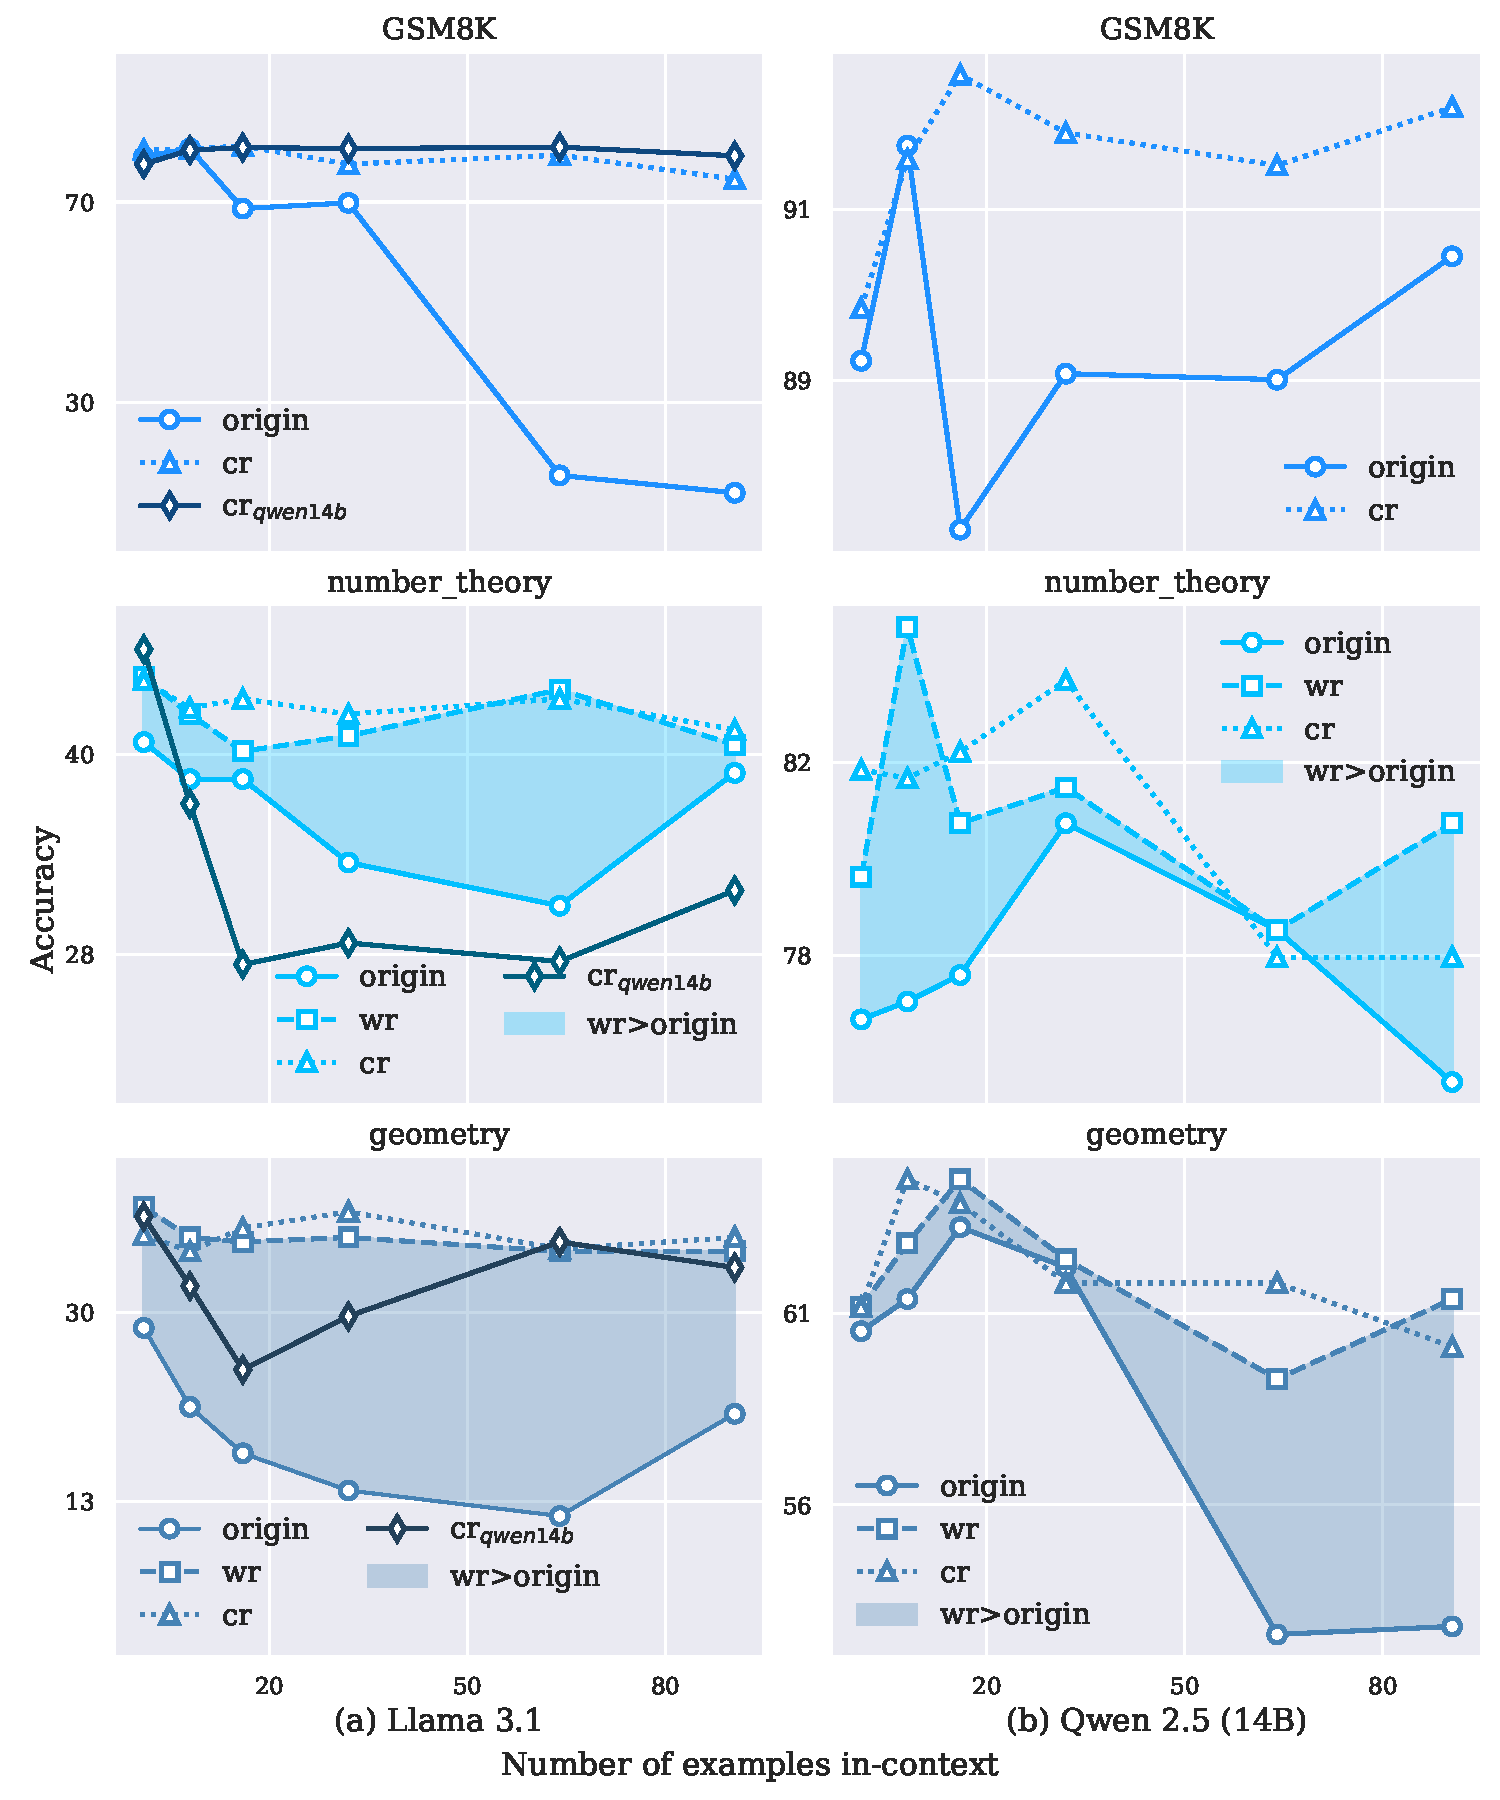
\includegraphics[width=\linewidth]{figures/selfgen_non_reasonng.pdf}
    \caption{Performance of two sets of self-generated in-context CoT, including the set filtered with only correct answer(cr) and the set filtered with only wrong answer(wr). cr$_\text{qwen14}$ is prompting the LLaMA model with the in-context CoT generated by Qwen 2.5 (14B). \emph{Left:} Llama 3.1 \emph{Right:} Qwen 2.5 (14B)}
    \label{fig:modelr}
    \vspace{-6mm}
\end{figure}


\begin{figure}[t]
    \centering
    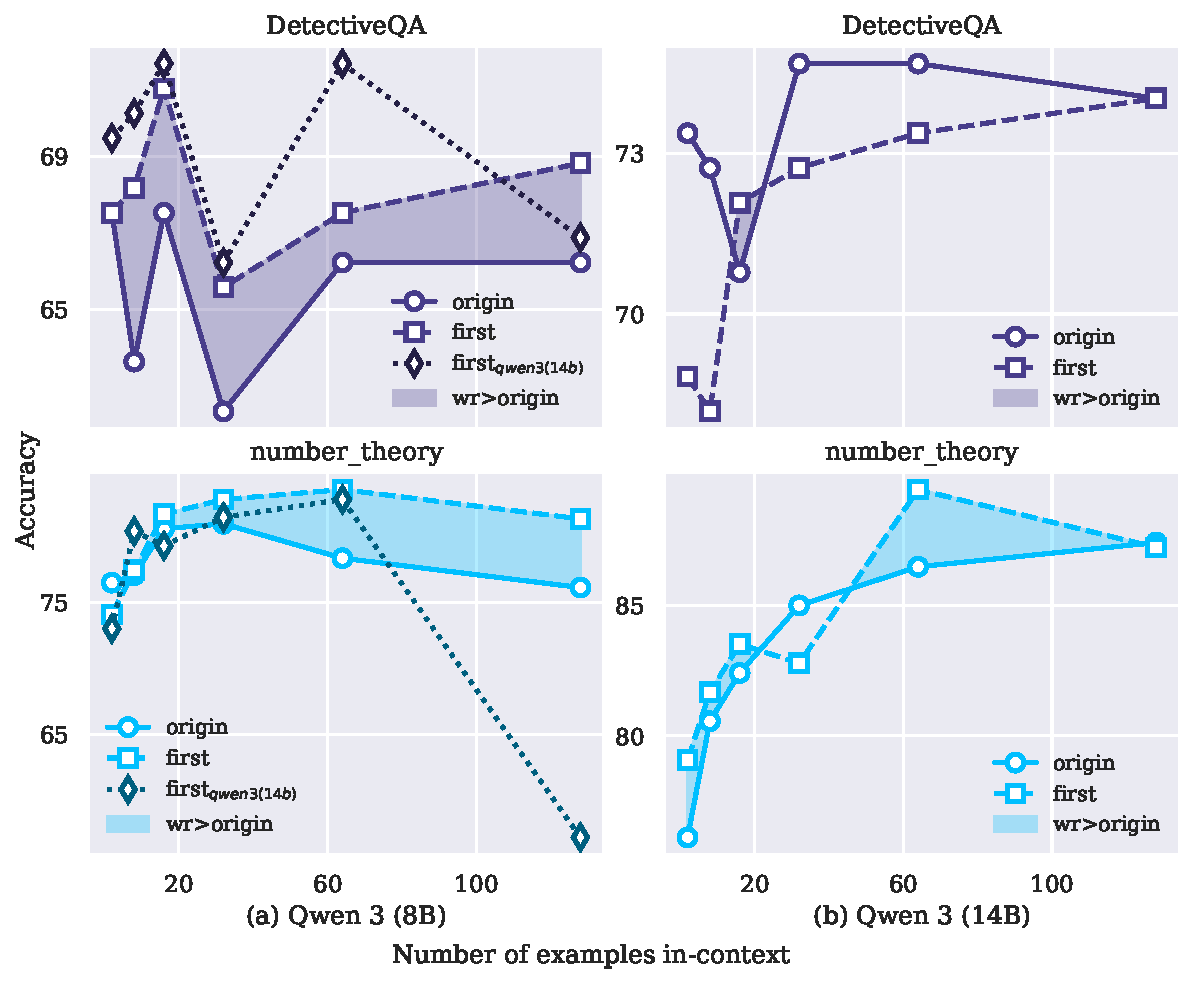
\includegraphics[width=\linewidth]{figures/selfgen_reasoning.pdf}
    \caption{Performance of the first set of self-generated in-context CoT. first$_\text{qwen3(14b)}$ is prompting the Qwen 3 (8B) model with the in-context CoT generated by Qwen 3 (14B). \emph{Left:} Qwen 3 (8B) \emph{Right:} Qwen 3 (14B)}
    \label{fig:modelfr}
    \vspace{-4mm}
\end{figure}
\vspace{-4mm}
\subsection{Principle 2: Smoothness of information flow}
\label{sec:curvature_corr}


Effective learning requires not just comprehensible individual examples, but a coherent progression between them. We hypothesize that smooth transitions between demonstrations facilitate the model's construction of a coherent reasoning schema, while abrupt conceptual jumps disrupt this process.
\subsubsection{Settings: Quantifying Transition Smoothness}

We measure smoothness by viewing an ordered list of demonstrations as a trajectory in embedding space.
We represent each demonstration $\mathbf{d}_i$ as \emph{(question + CoT + final answer)} and embed it using Qwen3-Embedding-4B to obtain $\mathbf{e}_i \in \mathbb{R}^d$.
Unlike Section~\ref{sec:sim} (question-only similarity), we embed the full demonstration because ordering effects should depend on procedural content.
This representation is designed to capture not only topical similarity but also the logical structures and operations expressed in the CoT rationale.
For efficient and stable curvature estimation, we compute curvature in a projected space obtained from the set of embeddings in the prompt with details in Appendix~\ref{sec:algocurvature}.
Let $\tilde{\mathbf{e}}_i \in \mathbb{R}^{d'}$ denote the projected embedding of $\mathbf{e}_i$.


Given an ordering $O=[\mathbf{d}_1,\dots,\mathbf{d}_n]$, we define local curvature at position $i$ as the turning angle between consecutive displacement vectors:
\begin{equation}
\theta_i
=
\arccos\left(
\frac{(\tilde{\mathbf{e}}_{i} - \tilde{\mathbf{e}}_{i-1}) \cdot (\tilde{\mathbf{e}}_{i+1} - \tilde{\mathbf{e}}_{i})}
{\|\tilde{\mathbf{e}}_{i} - \tilde{\mathbf{e}}_{i-1}\|\;\|\tilde{\mathbf{e}}_{i+1} - \tilde{\mathbf{e}}_{i}\|}
\right)
\end{equation}
Total curvature is $\Theta(O)=\sum_{i=2}^{n-1}\theta_i$, where smaller values indicate smoother transitions.
Implementation details (including the exact concatenation template and robustness checks) are in Appendix~\ref{sec:algocurvature}.

\subsubsection{Results}
Across three math reasoning tasks, ordering curvature is strongly negatively correlated with accuracy: overall $r=-0.547$, with task-wise correlations of $-0.545$ (geometry), $-0.468$ (number\_theory), and $-0.628$ (counting\_and\_probability).
Thus, smoother orderings tend to yield better performance.

This also provides a concrete explanation for the increasing order variance observed in Section~\ref{sec:variance}.
As the number of demonstrations grows, random permutations are more likely to contain sharp ``conceptual jumps'' (high curvature), amplifying variability across orders.
Controlling the ordering to reduce curvature yields a more stable learning trajectory, motivating our ordering method in Section~\ref{sec:CDS}.

\paragraph{Causal smoothness ablation.}
To separate smooth transitions from local clustering, we construct two orderings from the same demonstrations using bge-m3 embeddings.
Both orderings constrain Euclidean proximity, but the high-curvature baseline inverts the curvature objective, forcing abrupt conceptual turns while preserving local neighborhoods.
Across number\_theory and geometry, CDS consistently outperforms this high-curvature ordering in Table ~\ref{tab:high_curvature_ablation}, supporting transition smoothness as a causal factor rather than a by-product of grouping similar examples.










\subsubsection{Discussion: Pedagogical Analogy} This principle mirrors effective textbook design: concepts are introduced progressively, with each chapter building smoothly upon the previous. Abrupt topic changes or missing prerequisites hinder learning. Similarly, in many-shot CoT-ICL, demonstrations must be ordered to create a "conceptual curriculum" that guides the model from basic to advanced reasoning steps.






